\documentclass[aspectratio=169,12pt]{beamer}
\usetheme{default}
\usepackage[T1]{fontenc}
\usepackage{lmodern}
\usepackage{amsmath,amssymb}
\usepackage{listings}
\usepackage{xcolor}
\usepackage{array}
\usepackage{booktabs}
\usepackage{tikz}
\usetikzlibrary{positioning,arrows.meta,fit,backgrounds,calc}

\definecolor{ink}{HTML}{1A1A1A}
\definecolor{pale}{HTML}{F5F3EE}
\definecolor{seq}{HTML}{1F4E8C}
\definecolor{grey}{HTML}{5F5B54}
\definecolor{tensor}{HTML}{1F6F4A}
\definecolor{prod}{HTML}{9C3B1B}
\definecolor{kw}{RGB}{20,80,160}
\definecolor{cmt}{RGB}{110,110,110}
\definecolor{codebg}{RGB}{246,246,244}

\setbeamercolor{background canvas}{bg=pale}
\setbeamercolor{normal text}{fg=ink}
\setbeamercolor{frametitle}{fg=seq, bg=}
\setbeamerfont{frametitle}{size=\Huge, series=\bfseries}
\setbeamertemplate{navigation symbols}{}
\setbeamertemplate{frametitle}{\vspace{1em}\centering\insertframetitle\par}

\tikzset{
  srv/.style={draw=ink, fill=white, rounded corners=2pt, inner sep=3.4pt,
              font=\scriptsize\ttfamily, minimum height=5.6mm},
  plan/.style={srv, fill=pale, font=\scriptsize\ttfamily\bfseries},
  op/.style={circle, draw, inner sep=0.6pt, minimum size=6.4mm, font=\footnotesize\bfseries},
  ar/.style={-{Stealth[length=1.8mm]}, semithick, color=grey},
  lbl/.style={font=\tiny\itshape, color=grey},
  capt/.style={font=\scriptsize\bfseries},
  subt/.style={font=\tiny\itshape, color=grey},
}

\lstdefinelanguage{TS}{
  morekeywords={const,await,return},
  sensitive=true,
  morecomment=[l]{//},
}
\lstset{
  language=TS,
  basicstyle=\ttfamily\small,
  keywordstyle=\color{kw}\bfseries,
  commentstyle=\color{cmt}\itshape,
  backgroundcolor=\color{codebg},
  frame=leftline,
  framesep=7pt,
  xleftmargin=10pt,
  rulecolor=\color{gray!45},
  columns=fullflexible,
  showstringspaces=false,
  keepspaces=true,
  aboveskip=0pt, belowskip=0pt,
}

\newcommand{\slidebody}[1]{%
  \vfill
  \begin{center}\begin{minipage}{0.86\textwidth}\centering\Large #1\end{minipage}\end{center}
  \vfill}

\begin{document}

\begin{frame}
\vfill
\begin{center}
\begin{minipage}{0.92\textwidth}
\raggedright
\large

Neil Ghani's \emph{Containers for Typed Agentic AI} describes an algebra of interfaces. An
interface is a pair. The first half is the prompts you may send. The second half gives, for each
prompt, the type of response that would answer it.

\medskip

Such interfaces compose, in four different ways. Three of them appear in this game.

\end{minipage}
\end{center}
\vfill
\end{frame}

\begin{frame}
\vfill
\begin{center}
\begin{minipage}{0.94\textwidth}
\raggedright

\begin{tabular}{@{}c@{\hspace{4mm}}l@{\hspace{4mm}}>{\raggedright\arraybackslash}p{0.62\textwidth}@{}}
\toprule
& & \\[-3.4mm]
{\large\color{tensor}$\boxtimes$} & \textbf{tensor}     & prompts both sides, and requires a response from each \\[1.6mm]
{\large\color{seq}$\lhd$}         & \textbf{sequential} & prompts one side, and computes the second prompt from the first response \\[1.6mm]
{\large\color{prod}$\times$}      & \textbf{product}    & offers both sides, and takes a response from exactly one \\[1.6mm]
{\large$+$}                       & \textbf{sum}        & takes a prompt belonging to one side or the other, and answers with that side's own response \\[-0.6mm]
\bottomrule
\end{tabular}

\medskip

The sum is routing. We only use the first three in this game.

\end{minipage}
\end{center}
\vfill
\end{frame}

\begin{frame}
\vfill
\begin{center}
\begin{minipage}{0.92\textwidth}
\raggedright
\large

A morphism of containers $(P, R) \to (Q, T)$ is a pair of functions.

\medskip

\[
u : P \to Q
\qquad\qquad
f : (p : P) \to T\,(u\,p) \to R\,p.
\]

\medskip

The mapping $u$ delegates a task. The mapping $f$ amalgamates a response. So a container morphism
has two flows, prompts moving forwards and responses moving backwards.

\medskip

Control flows \emph{down} through $u$. Data flows \emph{back up} through $f$.

\end{minipage}
\end{center}
\vfill
\end{frame}

\begin{frame}
\vfill
\begin{center}
\begin{minipage}{0.92\textwidth}
\raggedright
\large

\textbf{CLI tools:} The forward map $u$ on shapes is implemented as a Unix CLI tool call.

\medskip

This works because a command-line tool is already a container. It receives one prompt, its
argument vector. It produces a response whose \emph{type depends on which prompt it was}.

\bigskip

\textbf{TypeScript \texttt{async} event handlers:} The backwards map $f$ on positions is
implemented with TypeScript \texttt{async} event handlers.

\end{minipage}
\end{center}
\vfill
\end{frame}

\begin{frame}
\frametitle{Typed agents}
\vfill
\begin{center}
\begin{minipage}{0.92\textwidth}
\raggedright
\large

Note that the Claude Code harness is itself a CLI tool, and thus a container. We can simply
``plug in'' the \texttt{claude} binary as our CLI tool, and all the machinery developed in this
note works exactly the same.

\end{minipage}
\end{center}
\vfill
\end{frame}

\begin{frame}
\frametitle{A note on formal verification}
\vfill
\begin{center}
\begin{minipage}{0.92\textwidth}
\raggedright
\large

The architecture of the game is motivated by Ghani's theory of container combinators, but the
design is not formally verifiable. This was never the point. It is a ``fake'', but it is a fake
that works.

\end{minipage}
\end{center}
\vfill
\end{frame}

\begin{frame}
\frametitle{Stalin: The Game}
\vfill
\begin{center}
\begin{minipage}{0.92\textwidth}
\raggedright
\large

This is a game about Stalin and his First Five-Year Plan. You are given the Soviet Union in 1928
and five years to industrialise it. You must also win the war in 1941.

\medskip

This was a tragic episode of history and I don't wish to make light of the story. It is for
illustrative purposes only. It is also a history lesson.

\end{minipage}
\end{center}
\vfill
\end{frame}

\begin{frame}
\vfill
\begin{center}
\resizebox{!}{0.86\textheight}{%
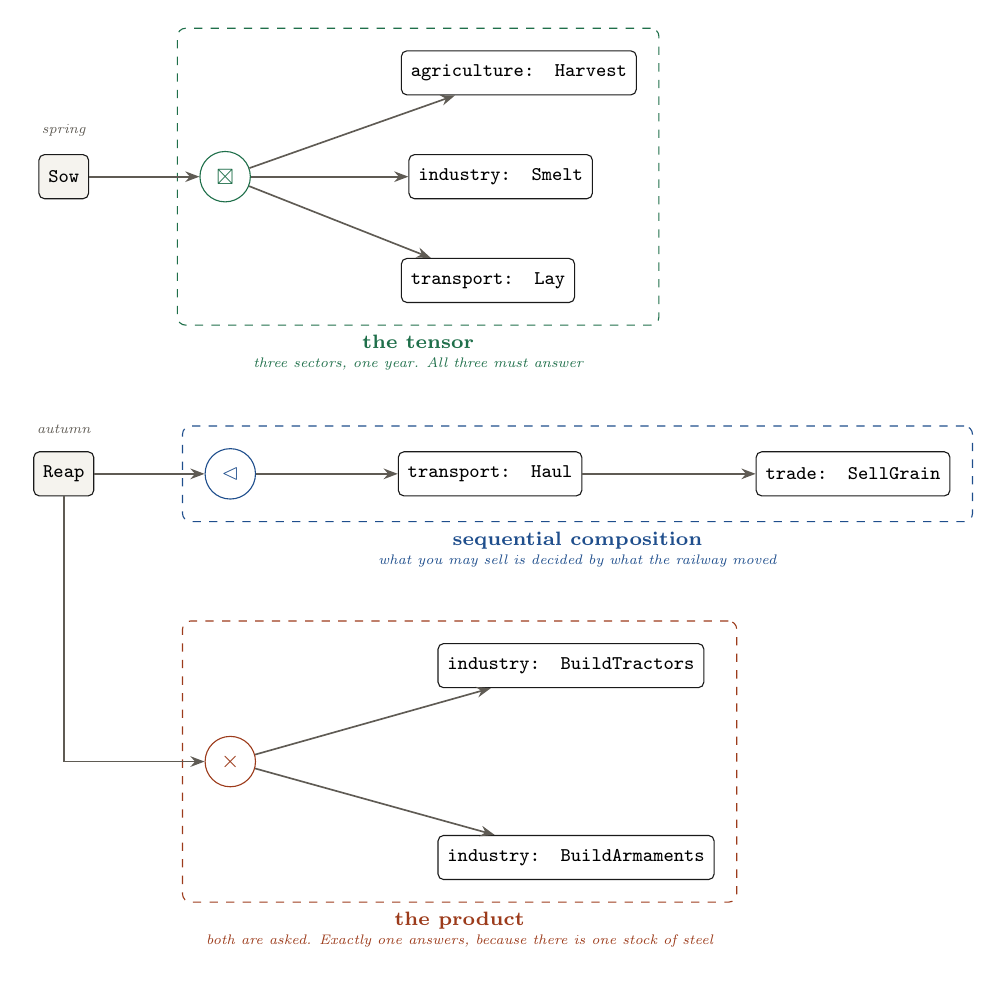
\begin{tikzpicture}
% --- SPRING: tensor ---
\node[plan] (sow) {Sow};
\node[lbl, above=1mm of sow] {spring};
\node[op, draw=tensor, text=tensor] (t1) [right=14mm of sow] {$\boxtimes$};
\node[srv] (agri)  [above right=8mm and 20mm of t1] {agriculture: Harvest};
\node[srv] (mill)  [right=20mm of t1]               {industry: Smelt};
\node[srv] (rail)  [below right=8mm and 20mm of t1] {transport: Lay};
\draw[ar] (sow) -- (t1);
\draw[ar] (t1) -- (agri);
\draw[ar] (t1) -- (mill);
\draw[ar] (t1) -- (rail);
\begin{scope}[on background layer]
\node[fit=(t1)(agri)(mill)(rail), draw=tensor, dashed, rounded corners=3pt,
      inner sep=2.8mm, label={[capt, text=tensor, align=center]below:%
      the tensor\\[-0.4mm]
      {\normalfont\itshape\tiny three sectors, one year. All three must answer}}] {};
\end{scope}

% --- AUTUMN: seq ---
\node[plan] (reap) [below=32mm of sow] {Reap};
\node[lbl, above=1mm of reap] {autumn};
\node[op, draw=seq, text=seq] (s1) [right=14mm of reap] {$\lhd$};
\node[srv] (rail2) [right=18mm of s1]    {transport: Haul};
\node[srv] (trade) [right=22mm of rail2] {trade: SellGrain};
\draw[ar] (reap) -- (s1);
\draw[ar] (s1) -- (rail2);
\draw[ar] (rail2) -- (trade);
\begin{scope}[on background layer]
\node[fit=(s1)(rail2)(trade), draw=seq, dashed, rounded corners=3pt,
      inner sep=2.8mm, label={[capt, text=seq, align=center]below:%
      sequential composition\\[-0.4mm]
      {\normalfont\itshape\tiny what you may sell is decided by what the railway moved}}] {};
\end{scope}

% --- PRODUCT ---
\node[op, draw=prod, text=prod] (p1) [below=30mm of s1] {$\times$};
\node[srv] (tract) [above right=7mm and 24mm of p1] {industry: BuildTractors};
\node[srv] (arms)  [below right=7mm and 24mm of p1] {industry: BuildArmaments};
\draw[ar] (reap) |- (p1);
\draw[ar] (p1) -- (tract);
\draw[ar] (p1) -- (arms);
\begin{scope}[on background layer]
\node[fit=(p1)(tract)(arms), draw=prod, dashed, rounded corners=3pt,
      inner sep=2.8mm, label={[capt, text=prod, align=center]below:%
      the product\\[-0.4mm]
      {\normalfont\itshape\tiny both are asked. Exactly one answers, because there is one stock of steel}}] {};
\end{scope}

\end{tikzpicture}}
\end{center}
\vfill
\end{frame}

\begin{frame}
\frametitle{Everything is a file}
\vfill
\begin{center}
\begin{minipage}{0.92\textwidth}
\raggedright
\large

An actual file on a disk, a terminal, a network connection, a source of random bytes. All of them
are presented by the kernel to user space through the same interface. So the same two calls reach
all of them.

\end{minipage}
\end{center}
\vfill
\end{frame}

\begin{frame}[fragile]
\frametitle{That interface to the kernel}
\vfill
\begin{center}
\begin{minipage}{0.72\textwidth}

\begin{lstlisting}[basicstyle=\ttfamily\large,morekeywords={read,write}]
read (n, buffer, count)
write(n, buffer, count)
\end{lstlisting}

\vspace{1.2em}

{\large The argument \texttt{n} is the file descriptor.\par}

\end{minipage}
\end{center}
\vfill
\end{frame}

\begin{frame}
\frametitle{The shell}
\vfill
\begin{center}
\begin{minipage}{0.92\textwidth}
\raggedright
\large

The shell is not part of the kernel and has no privilege you do not have. It is an ordinary
process running in user space with your identity, and its purpose is to start other processes.
That is all it is. A process whose job is starting other processes.

\end{minipage}
\end{center}
\vfill
\end{frame}

\begin{frame}
\frametitle{Pipes}
\vfill
\begin{center}
\begin{minipage}{0.92\textwidth}
\raggedright
\large

A pipe is a buffer the kernel will hand out on request. It comes with two descriptors. One to
write into, one to read out of. The symbol \texttt{|} is the same redirection as \texttt{>}, with
a pipe where the file was. The shell asks for a pipe, forks twice, puts the writing end in the
left program's slot 1 and the reading end in the right program's slot 0, and execs both.

\end{minipage}
\end{center}
\vfill
\end{frame}

\begin{frame}
\frametitle{The Unix philosophy}
\vfill
\begin{center}
\begin{minipage}{0.86\textwidth}
\centering
\Large

Write programs that do one thing and do it well.

\medskip

Write programs to work together.

\medskip

Write programs to handle text streams, because that is a universal interface.

\end{minipage}
\end{center}
\vfill
\end{frame}

\begin{frame}
\vfill
\begin{center}
\begin{minipage}{0.92\textwidth}
\raggedright
\large

\textbf{A CLI tool is already a container.}

\medskip

A command-line tool receives one prompt, its argument vector. It produces a response whose
\emph{type depends on which prompt it was}.

\medskip

For example the command \texttt{git log} answers with a list of commits. The command
\texttt{git status} answers with a working tree. Those are not the same kind of thing, and which
kind you get is fixed by the word after \texttt{git}.

\medskip

The interface is documented in the man pages. But there is \emph{no type checker}. Nothing
verifies whether the output from one CLI tool piped into the input of another has the right type.

\end{minipage}
\end{center}
\vfill
\end{frame}

\begin{frame}
\frametitle{Deliberately simple}
\vfill
\begin{center}
\begin{minipage}{0.92\textwidth}
\raggedright
\large

The designer of the HTTP protocol, Roy Fielding, made the same kind of design decision that Unix
made. And it paid off. Just as every server in the world today runs Unix, every web app in the
world today communicates via HTTP.

\end{minipage}
\end{center}
\vfill
\end{frame}

\begin{frame}
\vfill
\begin{center}
\begin{minipage}{0.92\textwidth}
\raggedright
\large

There are four types of HTTP request. We only use two of them.

\medskip

\begin{center}
\begin{tabular}{ll}
\toprule
\textbf{Method} & \textbf{Means} \\
\midrule
\texttt{GET}  & read something, change nothing \\
\texttt{POST} & create something \\
\bottomrule
\end{tabular}
\end{center}

\medskip

A simple web app runs a database on the server. When the server receives a \texttt{GET} request it
reads the database and returns the result to the client, or returns an error. When the server
receives a \texttt{POST} request it either writes to the database or returns an error.

\end{minipage}
\end{center}
\vfill
\end{frame}

\begin{frame}
\vfill
\begin{center}
\begin{minipage}{0.92\textwidth}
\raggedright

The command \texttt{curl} is just another Unix CLI tool. It sends one HTTP request across the wire
and prints the response to the standard output.

\medskip

Note that since ``everything is a file'' the Unix kernel handles all the networking, and
\texttt{curl} just thinks it is reading to and writing from a file.

\medskip

We say that the server is ``listening'' on port 8099. What this really means is that the kernel
has created a socket with unique ID number 8099 and handed it as a unique file descriptor to the
server. The kernel handles all the networking and the server thinks it is reading and writing to a
file. So we can forget about ``the wire''.

\medskip

This is very similar to a Unix pipe.

\end{minipage}
\end{center}
\vfill
\end{frame}

\begin{frame}[fragile]
\vfill
\begin{center}
\begin{minipage}{0.92\textwidth}
\raggedright
\large

JSON is short for JavaScript Object Notation. It is a recursive text format for data. Just like
HTTP it is deliberately simple. It has four types of ``atomic'' data: numbers, strings, booleans
and null. Then it has two recursive constructors: array and object.

\medskip

\begin{lstlisting}[basicstyle=\ttfamily\small]
value ::= string | number | boolean | null
        | '[' value* ']'
        | '{' (string ':' value)* '}'
\end{lstlisting}

\end{minipage}
\end{center}
\vfill
\end{frame}

\begin{frame}
\frametitle{Unchecked types}
\vfill
\begin{center}
\begin{minipage}{0.92\textwidth}
\raggedright
\large

A CLI interface is documented in the man pages, and nowhere enforced.

\medskip

The same is true one level up. The interface between the CLI tool making an HTTP request and the
TypeScript handler that answers it is fully specified in the design spec, and nowhere enforced.

\medskip

It must be maintained by the developer.

\end{minipage}
\end{center}
\vfill
\end{frame}


\begin{frame}
\vfill
\begin{center}
\begin{minipage}{0.92\textwidth}
\raggedright
\large

The design used by \texttt{deno} keeps one flow of control and never lets it block. Every
operation that would have waited is written in three parts instead.

\medskip

\begin{enumerate}\setlength{\itemsep}{0.4em}
\item Start it. Ask for the thing, and do not wait for it.
\item Give the flow of control back. Stop, so that the other conversations can be served.
\item Arrange to be resumed. Leave behind what should happen when the response arrives.
\end{enumerate}

\medskip

Something has to hold those arrangements. That something is the event loop.

\end{minipage}
\end{center}
\vfill
\end{frame}

\begin{frame}
\frametitle{Async hell}
\vfill
\begin{center}
\begin{minipage}{0.92\textwidth}
\raggedright
\large

Functions which depend on other functions which in turn depend on other functions form a tree.
Depending on how long each function takes to complete, they may return in any order which is a
linear extension of that tree.

\medskip

For a complex dependency tree, writing out all the \texttt{async} and \texttt{await} keywords to
record the nesting structure is a nightmare. It is commonly referred to as async hell. This is
exactly the problem that Ghani's container formalism solves.

\end{minipage}
\end{center}
\vfill
\end{frame}

\begin{frame}
\vfill
\begin{center}
\begin{minipage}{0.92\textwidth}
\raggedright
\large

The tree is a dependency order, which is a partial order. The event loop produces some topological
sort of it, and which one you get is decided by whichever promise settles first.

\medskip

That is the gap the four combinators close. The tensor $\boxtimes$ says that two subtrees are
independent and may interleave. The sequential $\lhd$ says that one must precede the other. The
combinators are a language for writing down the partial order, so you no longer have to
hand-schedule a linear one.

\end{minipage}
\end{center}
\vfill
\end{frame}

\begin{frame}[fragile]
\vfill
\begin{center}
\begin{minipage}{0.92\textwidth}
\raggedright
\large

The three fields of a \texttt{Book} form a finite union:

\medskip

\begin{lstlisting}[basicstyle=\ttfamily\small,morekeywords={type}]
type Field = "id" | "title" | "author";
\end{lstlisting}

\medskip

Notice that the three fields do not hold the same kind of thing. An id is a number. A title
and an author are strings. That fact can be written down as a function, on the level of types.

\medskip

\begin{lstlisting}[basicstyle=\ttfamily\small,morekeywords={type,extends}]
type FieldType<F extends Field> =
  F extends "id" ? number : string;
\end{lstlisting}

\end{minipage}
\end{center}
\vfill
\end{frame}

\begin{frame}[fragile]
\vfill
\begin{center}
\begin{minipage}{0.92\textwidth}
\raggedright
\large

The function below returns a book field. Its result type is calculated from which field you
ask for. It looks a little bit
like a dependent type, but that is not quite what it is.

\medskip

\begin{lstlisting}[basicstyle=\ttfamily\small,morekeywords={function,return,const,as,extends}]
function field<F extends Field>(b: Book, f: F): FieldType<F> {
  return b[f] as FieldType<F>;
}

const n = field(book, "id");      // n : number
const s = field(book, "title");   // s : string
const t = field(book, "author");  // t : string
\end{lstlisting}

\end{minipage}
\end{center}
\vfill
\end{frame}

\begin{frame}
\frametitle{The fake container}
\vfill
\begin{center}
\begin{minipage}{0.92\textwidth}
\raggedright
\large

An interface is a pair. The prompts you may send, and for each prompt the type of response it can
receive.

\medskip

Here \texttt{Field} is the type of the prompts, and \texttt{FieldType} is the type of the response
for each prompt.

\medskip

So \texttt{(Field, FieldType)} is a container, and \texttt{field} is an inhabitant of it.

\end{minipage}
\end{center}
\vfill
\end{frame}

\begin{frame}
\frametitle{Everything is a CLI tool}
\vfill
\begin{center}
\begin{minipage}{0.92\textwidth}
\raggedright
\large

The TypeScript web server \texttt{deno} is itself a CLI tool, and it can execute other CLI tools.
Claude himself is a large language model running on Anthropic's servers. The Claude Code harness
is something else entirely. It is a TypeScript program running on Unix as a CLI tool. So
\texttt{deno} can delegate to Claude Code.

\end{minipage}
\end{center}
\vfill
\end{frame}

\begin{frame}
\frametitle{Formal verifiability}
\vfill
\begin{center}
\begin{minipage}{0.92\textwidth}
\raggedright

The short answer is that this design cannot be formally verified. The algebra motivates the
architecture. It does not verify it.

\medskip

The algebra is a design vocabulary, and it was used as one.

\medskip

The algebra is the reason the game is five processes rather than one. A morphism has a level
above and a level below, and making the boundary a socket makes that claim falsifiable.

\medskip

The algebra is the reason each turn is a named composite rather than a block of code. The
algebra offers four ways to combine, and forces the designer to say which.

\end{minipage}
\end{center}
\vfill
\end{frame}

\begin{frame}
\vfill
\begin{center}
\begin{minipage}{0.90\textwidth}
\centering
\large

The game runs as five programs, each listening on a port. The player talks only to the Plan. The
Plan delegates to the four commissariats beneath it.

\bigskip

\resizebox{\textwidth}{!}{%
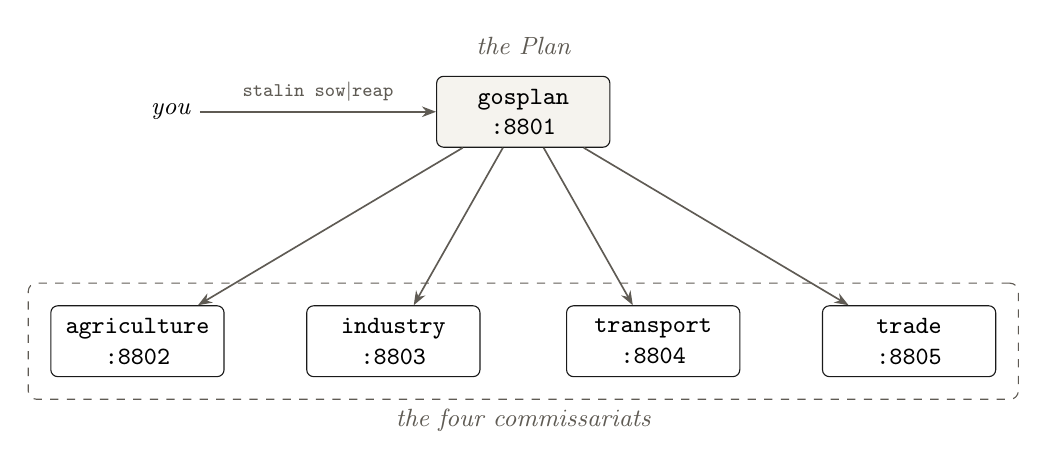
\begin{tikzpicture}[
  box/.style={draw=ink, fill=white, rounded corners=2.5pt, align=center,
              font=\small\ttfamily, inner sep=4.5pt, minimum width=22mm,
              minimum height=9mm},
]

\node[box, fill=pale, font=\small\ttfamily\bfseries] (gos) {gosplan\\:8801};
\node[lbl, above=1.5mm of gos, font=\small\itshape] {the Plan};
\node[font=\small\itshape] (you) [left=30mm of gos] {you};
\draw[ar] (you) -- node[above, pos=0.5, font=\scriptsize\ttfamily]{stalin sow$\mid$reap} (gos);

\node[box] (agri)  [below=20mm of gos, xshift=-49mm] {agriculture\\:8802};
\node[box] (ind)   [below=20mm of gos, xshift=-16.5mm] {industry\\:8803};
\node[box] (tran)  [below=20mm of gos, xshift= 16.5mm] {transport\\:8804};
\node[box] (trade) [below=20mm of gos, xshift= 49mm] {trade\\:8805};

\draw[ar] (gos) -- (agri);
\draw[ar] (gos) -- (ind);
\draw[ar] (gos) -- (tran);
\draw[ar] (gos) -- (trade);

\begin{scope}[on background layer]
\node[fit=(agri)(ind)(tran)(trade), draw=grey, dashed, rounded corners=3pt,
      inner sep=2.8mm, label={[subt, font=\small\itshape]below:the four commissariats}] {};
\end{scope}

\end{tikzpicture}}

\end{minipage}
\end{center}
\vfill
\end{frame}

\begin{frame}
\frametitle{Conclusion}
\slidebody{%
What has been built is a \emph{fake}. Containers for event-driven programming, faked with CLI
tools and TypeScript \texttt{async} event handlers.

\bigskip

The nicest thing about this fake is that you can substitute \texttt{claude} for any of the CLI
tools.
}
\end{frame}

\begin{frame}[fragile]
\vfill
\begin{center}
\begin{minipage}{0.90\textwidth}

The impersonation has three parts.

\medskip

\begin{itemize}\setlength{\itemsep}{0.7em}

\item A container $(P, R)$ becomes a tagged union together with a lookup indexed by its tags. That
works, and works only, because the tag set is \emph{finite}. Over a finite index a dependent type
is just a table, and a table is something TypeScript can write down.

\item The inhabitant $(p : P) \to R\,p$ becomes the handler record. The compiler enforces its
totality, because it is a mapped type over that same union.

\item A morphism becomes an \texttt{async} function. That is where the two directions meet.

\end{itemize}

\medskip

\begin{lstlisting}[basicstyle=\ttfamily\footnotesize]
const reply = await lower.run(u(prompt));   // the prompt, going down
return f(prompt, reply);                    // the reply, coming back
\end{lstlisting}

\end{minipage}
\end{center}
\vfill
\end{frame}

\begin{frame}
\vfill
\begin{center}
\begin{minipage}{0.86\textwidth}
\centering
\setlength{\parindent}{0pt}
\Large

Even though this implementation of Ghani's container combinators is not formally verifiable in the
way that Kodamai would perhaps wish, Claude can still build lots of cool stuff with it.

\bigskip

Very quickly.

\end{minipage}
\end{center}
\vfill
\end{frame}

\end{document}
